
\documentclass{package/notes}
\usepackage[english]{babel}
\usepackage{amssymb,amsmath,amsfonts}  %%% for maths
%%%%%%%%%%%%%%%%%%%%%%%%%%%%%%%%%%%%%
\usepackage{package/color-env}
\usepackage{lipsum}
\usepackage{graphicx}
\renewcommand\qedsymbol{$\blacksquare$}
%%%%%%%%%%%%%%%%%%%%%%%%%%%%%%%%%%%%%

\begin{document}

	\begin{titlepage} % Suppresses headers and footers on the title page
		
		\centering % Centre everything on the title page
		
		\scshape % Use small caps for all text on the title page
		
		\vspace*{\baselineskip} % White space at the top of the page
		
		%------------------------------------------------
		%	Title
		%------------------------------------------------
		
		\rule{\textwidth}{1.6pt}\vspace*{-\baselineskip}\vspace*{2pt} % Thick horizontal rule
		\rule{\textwidth}{0.4pt} % Thin horizontal rule
		
		\vspace{0.75\baselineskip} % Whitespace above the title
		
		{\huge Multivariable Calculus\\} % Title
		
		\vspace{0.75\baselineskip} % Whitespace below the title
		
		\rule{\textwidth}{0.4pt}\vspace*{-\baselineskip}\vspace{3.2pt} % Thin horizontal rule
		\rule{\textwidth}{1.6pt} % Thick horizontal rule
		
		\vspace{2\baselineskip} % Whitespace after the title block
		
		%------------------------------------------------
		%	Subtitle
		%------------------------------------------------
		
		\LARGE{Public Notes for Any Multivariable Calculus Course} 
		
		\vspace*{3\baselineskip} % Whitespace under the subtitle
		
		
		
		\vspace{0.5\baselineskip} 
		
		\vspace{0.5\baselineskip} 
		
		
		\vfill 
		
		%------------------------------------------------
		% Author
		%------------------------------------------------
		
		
		\vspace{0.3\baselineskip} 
		
		
		{\large Edited by\\  Trevor Bushnell} 
		
	\end{titlepage}
	\tableofcontents
%\newpage
\chapter{Vectors and the Geometry of Space}

\section{3D Coordinate Systems}

\subsection{About 3D Coordinate Systems}
\begin{itemize}
	\item We are used to working in textbf{planes} (1D input and 1D output), and we can model each input and output on a 2D plane
	\item Multivariable calculus is all about representing points in \textbf{space} (2D input and 1D output)
	\item There are 2 \textit{axes} in 2D space $\to$ there are textbf{3 axes} in 3D space
	\item There are 4 \textit{quadrants} in 2D space $\to$ there are 8 \textbf{octants} in 3D space
	\item There is \textit{one plane} in 2D space ($xy$-plane) $\to$ there are \textbf{3 planes} in 3D space ($xy$-plane, $xz$-plane, and $yz$-plane)
	\item Points in 2D space have \textit{2 coordinates} $\to$ points in 3D space have \textbf{3 coordinates}
	\item We went from creating \textit{graphs} in 2D space to creating \textbf{surfaces} in 3D space
	\item If you have a hard time visualizing 3D space, use the room around you and pick a bottom corner in the room
	\begin{itemize}
		\item Floor is $xy$-plane
		\item Left wall is $xz$-plane
		\item Right wall is $yz$-plane
	\end{itemize}
\end{itemize}

\subsection{The Distance Formula (3D)}

\begin{itemize}
	\item Distance formula in 3D is very similar to the distance formula in 2D
	\item Finds the distance between point $P_1$ and $P_2$ 
\end{itemize}

\begin{definition}
	To find the distance between two points $P_1(x_1, y_1, z_1)$ and $P_2(x_2,y_2,z_2)$, use the following distance formula:
	$$D = \sqrt{(x_2-x_1)^2 + (y_2-y_1)^2 + (z_2-z_1)^2}$$
\end{definition}

\subsection{Equation of a Sphere}
We will be representing many surfaces and it is important to understand the different types of surfaces that we will encounter. A basic one is a sphere, which looks like the following:
\begin{proposition}
	The equation of a sphere with center $C(h,k,l)$ and radius $r$ is
	$$(x-h)^2 + (y-k)^2 + (r-l)^2 = r^2$$
\end{proposition}


\section{Vectors}

\subsection{About Vectors}

\begin{definition}
	A \textbf{vector} is a quantity that has both a \textit{direction} and a \textit{magnitude} (length).\\

Ex: 60mph North is a vector because it has a magnitude (60mph) and a direction (North)\\

We denote a vector by using either boldface ($\mathbf v$) or drawing an arrow over the name of the vector ($\vec v$)
\end{definition}

\begin{itemize}
	\item $\vec{O}$ is called the "zero vector and has length $0$ and no direction
\end{itemize}

\subsection{Vector Components and Magnitudes}
\begin{itemize}
	\item A vector algebraically looks like this $\to \vec{a} = <a_1, a_2>$ 
	\begin{itemize}
		\item The coordinates of $\vec a$ are the \textbf{components} of $\vec a$ 
	\end{itemize}
\end{itemize}

\begin{proposition}
	The algebraic representation of a vector between points $A(x_1, y_1, z_1)$ and B$(x_2, y_2,z_2)$ is
	$$\vec a = <x_2-x_1,y_2-y_1,z_2-z_1>$$\\

	To find the x-component of a vector, you can use the formula:
	$$\vec a_x = ||\vec a||\cos\theta$$\\

	To find the y-component of a vector, you can use the formula:
	$$\vec a_x = ||\vec a||\cos\theta$$\\

	Where $\theta$ is the angle between the vector and the x-axis
\end{proposition}

\begin{proposition}
	To find the magnitude of the vector $\vec a$, use the distance formula (2D in the case of working with vectors having 2 components, 3D in the case of working with vectors with 3 components):

	\begin{equation*}
		\begin{aligned}
			||\vec a|| =&\: \sqrt {a_1^2 + a_2^2 + a_3^2}\\
			&OR\\
			||\vec a|| =&\: \sqrt {a_1^2 + a_2^2}\\
		\end{aligned}
	\end{equation*}
\end{proposition}

\subsection{Adding Vectors}
\begin{itemize}
	\item TIP TO TAIL METHOD: Put the end of the second vector on the tip of the first vector \textit{without changing the direction of length}
	\begin{itemize}
		\item The vector connecting the tail of the first vector to the tip of the second vector is the sum of the two vectors
	\end{itemize}
	\item ALGEBRAICALLY: To add two vectors, add together their components
	\item To subtract two vectors, subtract their components
\end{itemize}

\subsection{Other Properties of Vectors}
\begin{itemize}
	\item To multiply a vector by a scalar (any number), multiply that scalar by each component of the vector
	\item Other properties of vectors can be found below: 
	
	\begin{figure*}[h]
		\begin{center}
			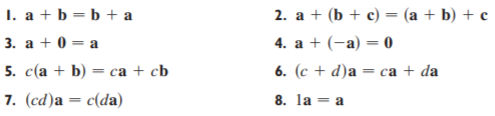
\includegraphics[width=10cm]{images/1.2.1_Image.PNG}
		\end{center}
	\end{figure*}
\end{itemize}

\subsection{Basis Vectors}
\begin{itemize}
	\item Vectors can also be written in relation to the unit vectors in the x, y, and z directions respectively (known as the \textbf{basis vectors})
\end{itemize}



\subsection{Applications}



\section{The Dot Product}

\subsection{Definition of the Dot Product}

\subsection{What Does the Dot Product Represent?}

\subsection{Direction Angles and Direction Cosines}



\section{The Cross Product}

\subsection{Definition of the Cross Product}

\subsection{What Does the Cross Product Represent?}

\subsection{Scalar Triple Products}

\subsection{Application: Torque}




\section{Equations of Lines and Planes}

\subsection{Lines in 3D}

\subsection{Planes}




\chapter{Partial Derivatives}



\chapter{Multiple Integrals}



\chapter{Vector Calculus}




\end{document}
.